\section{CAD Benchmark Tasks}
\label{sec:tasks}

BenchCAD comprehensively evaluates MLLMs’ CAD-related knowledge and their capabilities in understanding geometric structures and applying CadQuery to generate parametric models.
BenchCAD evaluates models on four tasks: \textsc{Vision QA}, \textsc{Code QA}, \textsc{Edit Code}, and \textsc{Vision2Code}.

\subsection{\textsc{Vision QA} and \textsc{Code QA}}
\label{sec:capability}

A per-family question bank asks only ratios and integer counts (never absolute mm) for scale invariance, with each item evaluated under both modalities --- visual (rendered views) and code-conditioned (CadQuery source). Scoring: relative error $\leq 5\%$ for ratios, exact match for integers.

We organise the QA bank along a four-level capability hierarchy (Figure~\ref{fig:capability_hierarchy}, left), from low-level perception at the base to high-level synthesis at the apex: \emph{(i) $L_1$ Holistic Visual Recognition} --- recognise the part family from multi-view renders and integrate views into a coherent volumetric understanding; \emph{(ii) $L_2$ CAD Operations Understanding} --- read CadQuery (or infer from geometry) and map operations to features in the right execution order; \emph{(iii) $L_3$ Industrial Parametric Abstraction} --- abstract observed geometry into the parametric structure an engineer would write, respecting standard-table relations and engineering conventions; \emph{(iv) $L_4$ Spatial/Code Reasoning} --- compose the lower three levels into syntactically valid, executable parametric code. The matched-pair design isolates the levels: a large $\texttt{qa\_img}-\texttt{qa\_code}$ gap on the same questions reveals the cost of replacing direct code access with visual recognition (the \textbf{Holistic Spatial and Detailing Deficit}, \S\ref{sec:exp_capability}); low absolute $\texttt{qa\_code}$ flags a \textbf{CAD Operational Blindspot} at $L_2$.

\begin{figure*}[t]
  \centering
  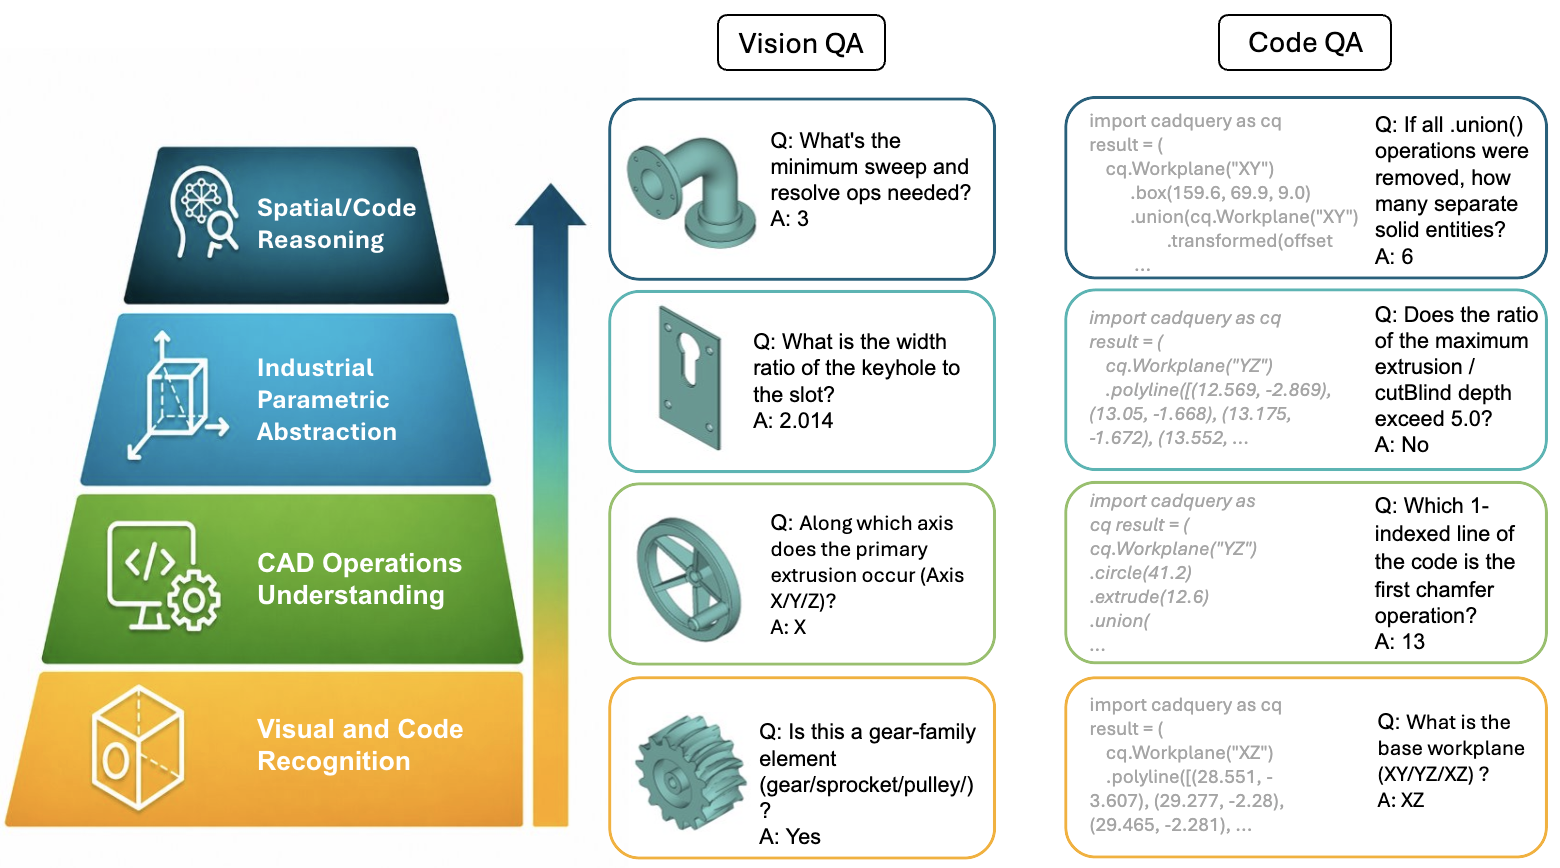
\includegraphics[width=0.75\linewidth]{figures/fig_6.png}
  \caption{\textbf{BenchCAD-QA capability hierarchy.} Four levels (L1 Holistic Visual Recognition $\to$ L4 Spatial/Code Reasoning) with paired \texttt{qa\_img} / \texttt{qa\_code} examples per level (\S\ref{sec:capability}).}
  \label{fig:capability_hierarchy}
\end{figure*}

\subsection{Instruction-Guided Editing: \texttt{edit\_code}}

Each item supplies an original CadQuery program, a natural-language edit instruction, and a target STEP, drawn from four categories (dimensional, additive, subtractive, multi-step). Pass@1 $= \mathbb{1}[\mathrm{IoU}(\text{edited},\text{target}) \geq 0.99 \wedge \mathrm{Preserve}(\text{edited},\text{orig}) \geq 0.99]$ requires both target-feature success \emph{and} non-target preservation. Disaggregating Pass@1 into the two component rates exposes the \textbf{Industrial Common Sense Gap} (\S\ref{sec:exp_edit}): a model can apply the requested change while silently corrupting unrelated parametric features.

\subsection{Image-to-Code Generation: \texttt{codegen}}

Four canonical orthographic views $\to$ executable CadQuery code. The codegen evaluation set comprises \textbf{350 stratified items spanning all 106 BenchCAD families} (full-family coverage, no family omitted). We report five metrics: \emph{(i)} \textbf{rotation-invariant IoU} between generated and ground-truth occupancy grids under the cube symmetry group, with $\mathrm{Pass}_{\mathrm{IoU}\geq 0.5}$ as the headline pass rate; \emph{(ii)} mean \textbf{Chamfer distance} between meshes after rigid alignment; \emph{(iii)} \textbf{Feature-F1}, precision/recall over detected geometric features (holes, fillets, chamfers, threads, $\ldots$); \emph{(iv)} \textbf{essential-op recall}, the fraction of items whose ground-truth program calls operation $o$ for which the model's emitted code also calls $o$ at least once (probing the Op Vocabulary Gap, Appendix~\ref{app:op_gap_full}); \emph{(v)} \textbf{execution rate}, the fraction of emitted programs that run without error. IoU is the primary metric; the other four disambiguate IoU ties and identify whether failures are geometric, structural, vocabulary-level, or syntactic.

The headline aggregate is the macro-mean across the four tasks. Question bank construction, edit-pair protocol, rotation-invariant IoU, and a scale-invariance ablation appear in Appendices~\ref{app:qbank}, \ref{app:edit_protocol}, \ref{app:iou}, and \ref{app:ablation} respectively.
